\documentclass[11pt]{article}
\usepackage[letterpaper, margin=1in]{geometry}
% \usepackage[skip=\baselineskip, tocskip=0pt]{parskip}
\usepackage{amsmath, amsfonts, amssymb, amsthm, mathtools}
\usepackage{stmaryrd}
\usepackage{fontspec}
\let\latextextsubscript\textsubscript
\AtBeginDocument{
  \let\textsubscript\latextextsubscript
  \newcommand{\sub}[1]{\textsubscript{#1}}
  \newcommand{\gap}[1]{\rule{1em}{0.4pt}\textsubscript{#1}}
}
\let\latextextsuperscript\textsuperscript
\AtBeginDocument{
  \let\textsuperscript\latextextsuperscript
}
\usepackage[largesc]{newpxtext}
\usepackage[vvarbb]{newpxmath}
\usepackage[threshold=1]{csquotes}
% \usepackage{markdown}

% \usepackage{pifont}
% \usepackage{txfonts}
\let\eachwordone=\rmfamily
\let\eachwordtwo=\rmfamily
\let\eachwordthree=\rmfamily
\let\rm=\relax
\usepackage[linguex]{expex-glossonly}
\lingset{everygla={\itshape}}
\renewcommand{\firstrefdash}{}
% \usepackage{hyperref}
% \usepackage{cleveref}
% \crefname{ExNo}{}{}
% \crefname{SubExNo}{}{}
% \renewcommand{\theExNo}{\arabic{ExNo}}
% \renewcommand{\theSubExNo}{\theExNo\alph{SubExNo}}
% \creflabelformat{SubExNo}{(#2#1#3)}
% \creflabelformat{ExNo}{(#2#1#3)}
% \crefrangelabelformat{SubExNo}{(#3#1#4--#5\crefstripprefix{#1}{#2}#6)}
% \crefrangelabelformat{ExNo}{(#3#1#4)--(#5#2#6)}
% \usepackage{enumitem}
% \usepackage[normalem]{ulem}
% \usepackage{xcolor}
%
% \usepackage{paracol}
% \usepackage{eqparbox}
% \setlength{\columnseprule}{.4pt}
% \globalcounter{ExNo}
\setlength{\parskip}{1ex}
\setlength{\parindent}{0pt}
% \setlist[1]{left=0pt}
% \renewcommand\thesection{\Roman{section}.}
% \renewcommand\thesubsection{\arabic{subsection}.}
% \renewcommand\thesubsubsection{\Alph{subsubsection}}

% \usepackage[
%   backend=biber,
%   natbib=true,
%   style=unified,
%   maxcitenames=3,
%   maxbibnames=99
% ]{biblatex}
% \addbibresource{../Distributivity.bib}
\AtBeginDocument{
  % \setlength{\Extopsep}{0\baselineskip}
  % \setlength{\Exredux}{0\baselineskip}
  \settowidth{\Exlabelwidth}{(00)}
  % \setlength{\Exlabelwidth}{.7\Exlabelwidth}
  % \setlength{\Exlabelsep}{.7\Exlabelsep}
  % \setlength{\SubExleftmargin}{\SubExleftmargin}
  % \setlength{\SubSubExleftmargin}{\SubSubExleftmargin}
}

\newcommand{\A}{\(\overline{\text{A}}\)}
% \usepackage{tikz}
\usepackage[linguistics]{forest}
% \usetikzlibrary{positioning}
% \usetikzlibrary{arrows.meta}
% \usetikzlibrary{tikzmark}
% \usepackage{tikz-cd}
% \tikzcdset{
%   arrow style=math font,
%   % diagrams={>={Straight Barb[scale=0.8]}}
% }
%
% \tikzset{every label/.style={font=\footnotesize}}
%
% \forestset{
%   default preamble={
%     for tree={
%       inner sep=0pt,
%       % draw,
%     }
%   },
%   great empty nodes/.style={
%     for tree={
%       calign=fixed edge angles,
%       calign primary angle=-60,
%       calign secondary angle=60, 
%     l=7mm},
%     delay={
%       where content={}{
%         shape=coordinate,
%     for current and siblings={anchor=north}}{}}
%   },
%   downroof/.style={
%     for children={
%       if n=1{
%         edge path'={
%           (.parent first) -- (!u.parent anchor) -- (!ul.parent last) -- cycle
%         }
%       }{no edge}
%     }
%   }
% }
% \usepackage{tabularx}
% \usepackage{booktabs}
% \renewcommand\tabularxcolumn[1]{m{#1}}% for vertical centering text in X column

\usepackage{langsci-avm}
\AtBeginDocument{% to do this after unicode-math has done its work
  \renewcommand{\setminus}{\mathbin{\backslash}}%
}
\title{Bar-Lev \& Fox (2020)}
\author{Haoming Li}
%
% \DeclareMathOperator{\atom}{\textsc{Atom}}
% \DeclareMathOperator{\alt}{\textsc{Alt}}
% \DeclareMathOperator{\xh}{\textsc{Exh}}
% \newcommand{\exh}{\ensuremath{\xh}}
% \newcommand{\Exh}{\ensuremath{\mathcal{E}\mathit{xh}}}
% \newcommand{\Pex}{\ensuremath{\mathcal{P}\mathit{ex}}}
% \DeclareMathOperator{\prt}{Part}
% \DeclareMathOperator{\dom}{dom}
% \newcommand{\dexh}{\ensuremath{D_{\textnormal{exh}}}}
% \newcommand{\dpart}{\ensuremath{D_{\textnormal{part}}}}
\begin{document}

\avmsetup{values=\normalfont,switch=*}
\section{SBCG (a dialect of HPSG)}
\label{sec:sbcg_a_dialect_of_hpsg}



\avm{
  [ mtr & [arg-st <NP\(_i\), S[mrkg \type{as-if}, syn|xarg NP[pron]\(_i\)]>] ]
}

The \textsc{xarg} feature talks about the external argument, like \textsc{spr} in HPSG; however, \textsc{xarg} is different from \textsc{spr} in that it is visible even after the merger with the external argument.

The \textsc{val(ence)} feature is like \textsc{arg-st} in HPSG, but with the difference that \textsc{arg-st} can contain `extracted' or unexpressed arguments, \textsc{val} does not.

\avm{
  [
    form & <\type{like}> \\
    syn & [
      cat & [
        \type{adverb} \\
        xarg & \type{none} \\
        select & [
          \type*{verb} \\
          syn & [
            cat & [
              vform & \type{fin} \\
              xarg & NP \\
              inv & \(-\)
            ] \\
            val & < & >
          ] \\
          sem & [
            ltop & \(l\) \\
            index & \(e\)
          ]
        ]
      ] \\
      val & < & > \\
      mrkg & \type{asif}
    ] \\
    sem & [
      frames & < *\type{as-if}\((e', l)\)* > \\
      index & \(e'\)
    ]
  ]
}


The following is a lexical rule in SBCG, another core of the analysis.
\avm{\(X\)! [A]} and \avm{\(X\):[B]} indicate that \avm{[A]} and \avm{[B]} are identical in all respects in which they are not shown to differ.

\avm{
  [
    mtr & \(X\)! [
      syn & [
        cat & [xarg \(Z\):NP\(_i\)] \\
        val & <\(Z\), [
          syn & [
            cat & [
              vform & \type{fin} \\
              xarg & NP[\type{pron}]\(_i\)
            ] \\
            val & < & > \\
            mrkg & \type{asif}
          ] \\
          sem & [
            ltop & \(l\)
          ]
        ]> \\
        sem & [
          frames & <*\type{seeming-fr}\((e)\)*, *\type{human-fr}\((j)\)*, \(l\)>\\
          index & \(e\)
        ]
      ]
    ] \\
    dtrs & <\(X\):[
      \type{verb} \\
      sem & [ frames & < *\type{gen-perception-fr}\((e)\)* > ]
    ]>
  ]
}

From a general perception predicate, one is able to derive a copy-raising predicate.

Semantically, copy-raising predicates involve a seeming event \(e\), and an experiencer \(j\).

Syntactically, copy-raising predicates requires a finite complement clause that has an external argument which is a pronoun; its own external argument must be co-indexed with the pronoun.

\ex. Trump looks like he disappeared.

\scalebox{0.8}{\begin{forest}
  for tree={fit=tight}
  [\avm{[
        form & <\type{trump,looks,like,he,disappeared}> \\
        syn & [
          cat & [
            \type*{verb} \\
            xarg & NP\(_i\) 
          ] \\
          val & < & > \\
          mrkg & \type{unmrk}
        ] \\
        sem & [
          frames & <*\(l_1\), \(l_2\), \(l_3\), \(l_4\)*>
        ]
    ]}
    [\avm{[
          form & <\type{trump}> \\
          syn & \type{pn-word} \\
          sem & [
            frames & <*\(l_4\)*, *\type{name-fr}\((i,\)\type{trump}\()\)*> \\
            index & \(i\)
          ]
    ]}]
    [\avm{[
          form & <\type{looks,like,he,disappeared}> \\
          syn & [
            cat & \\
            val & <\2> \\
            mrkg & \type{unmrk}
          ] \\
          sem & [
            frames & <*\(l_1\), \(l_2\), \(l_3\)*>
          ] \\
          cntxt & \3
      ]}
      [\avm{[
            form & <\type{looks}> \\
            syn & [
              cat & [
                \type{verb} \\
                xarg & \2 NP
              ] \\
              val & <\2, \4 S [
                mrkg & \type{asif} \\
                xarg & NP[\type{pron}]\(_i\)
              ]> \\
              mkrg & \type{unmrk}
            ] \\
            sem & [
              frames & <
              *\(l_3\): \type{generic-fr}\((j)\)*, & \\
              *\(l_3\): \type{human-fr}\((j)\)*, & \\
              *\(l_3\): \type{seeming-fr}\((e'', j, l_2)\)*, &\\
              *\(l_3\): \type{present-fr}\((e'')\)* & 
              > \\
              index & \(e''\)
            ]
      ]}]
      [\avm{[
            form & <\type{like,he,disappeared}> \\
            syn & [
              cat & [
                \type{verb} \\
                xarg & NP[\type{pron}]\(_i\)
              ] \\
              val & < & > \\
              mrkg & \type{asif}
            ] \\
            sem & [
              ltop & \(l_2\) \\
              frames & <*\(l_2\)*, *\(l_1\)*>
            ] \\
            cntxt & \3
          ]
        }
        [\avm{[
              form & <\type{like}> \\
              syn & [
                cat & [select & \1] \\
                mrkg & \type{asif}
              ] \\
              sem & [
                frames & <*\(l_2\): \type{as-if}\((e', l)\)*> \\
                index \(e'\)
              ]
        ]}]
        [\avm{[
              form & <\type{he,disappeared}> \\
              syn & [
                cat & [
                  \type{verb} \\
                  xarg & NP[\type{pron}]\(_i\)
                ] \\
                val & < & > \\
                mrkg & \type{unmrk}
              ] \\
              sem & [
                ltop & \(l_1\) \\
                frames & <
                *\(l_1\): \type{disappear-fr}\(e, i\)*, & \\
                *\(l_2\): \type{past-fr}\((e)\)* &
                > \\
                index & \(e\)
              ]
        ]}]
      ]
    ]
  ]
\end{forest}}

\section{LFG}
\label{sec:lfg}

Regular raising is simply achieved through structure sharing between the matrix subject and the open position of the complement, \textsc{xcomp}.
\ex. \begingl
  \gla It-tfal j-i-dhr-u (li) sejr-in tajjeb //
  \glb \textsc{def}-children 3-\textsc{frm.vwl}-appear.\textsc{impv-pl} \textsc{comp} go.\textsc{act.ptcp-pl} good //
  \glft `The children seem to be doing well' //
\endgl

Relevant features in the lexical entry for the raising predicate \emph{deher}:
\ex.  \begin{align*}
  (\uparrow \textsc{pred}) = \left\langle \textsc{xcomp} \right\rangle \textsc{subj} \\
  ((\uparrow \textsc{xcomp compform} = \textsc{li})) \\
  (\uparrow \textsc{subj}) = (\uparrow \textsc{xcomp subj}) \\
\end{align*}

\ex. \avm{[
    pred & `\emph{jidhru} <xcomp>\textsc{subj}' \\
    subj & \1 [
      pred & `\emph{tfal}' \\
      pers & 3 \\
      num & \textsc{pl} \\
      def & \(+\)
    ] \\
    xcomp & [
      pred & `\emph{sejrin} <subj>' \\
      subj & \1 \\
      adj & \{[
          pred & `\emph{tajjeb}'
      ]\}
    ]
]}

Now, copy-raising is slightly more involved: the matrix subject is still identified with with open position of the \textsc{xcomp}, but the identity relationship between these positions and the pronoun is not explicitly represented in the \(f\)-structure.

Rather, a semantic means ensures that the pronoun is abstracted away, turning the complement into a predicate of individuals; the matrix subject is then able to saturate this predicate.
\blockquote[Asudeh and Toivonen 2012]{
Asudeh (2002, 2004, 2012) provides an analysis of copy raising that assimilates the phenomenon to resumption, as centrally exemplified by resumptive pronouns in unbounded dependencies (McCloskey 1979, 1990, 2002, 2006; Sells 1984). 
On Asudeh’s analysis, the copy raising subject is not licensed by the copy raising verb and must instead compose in place of the copy pronoun, which is removed from semantic composition by a manager resource that is lexically contributed by the copy raising verb. 
Manager resources are somewhat analogous to empty operators that have independently been proposed for resumption (McCloskey 2002), but their logical status is quite different and they can be lexically controlled to an arguably greater extent (Asudeh 2004, 2012). 
In particular, a copy raising verb contributes a manager resource, whereas a perceptual resemblance verb does not. 
The analysis of the differ- ence between copy raising and perceptual resemblance with respect to the necessity of a pronoun is not a central concern in this paper, although we return to this difference briefly at a couple of points. 
We refer the reader to Asudeh’s work for further details and to the appendix of this paper for an example of a manager resource in a semantic proof.
}
\ex. John seems like he won.

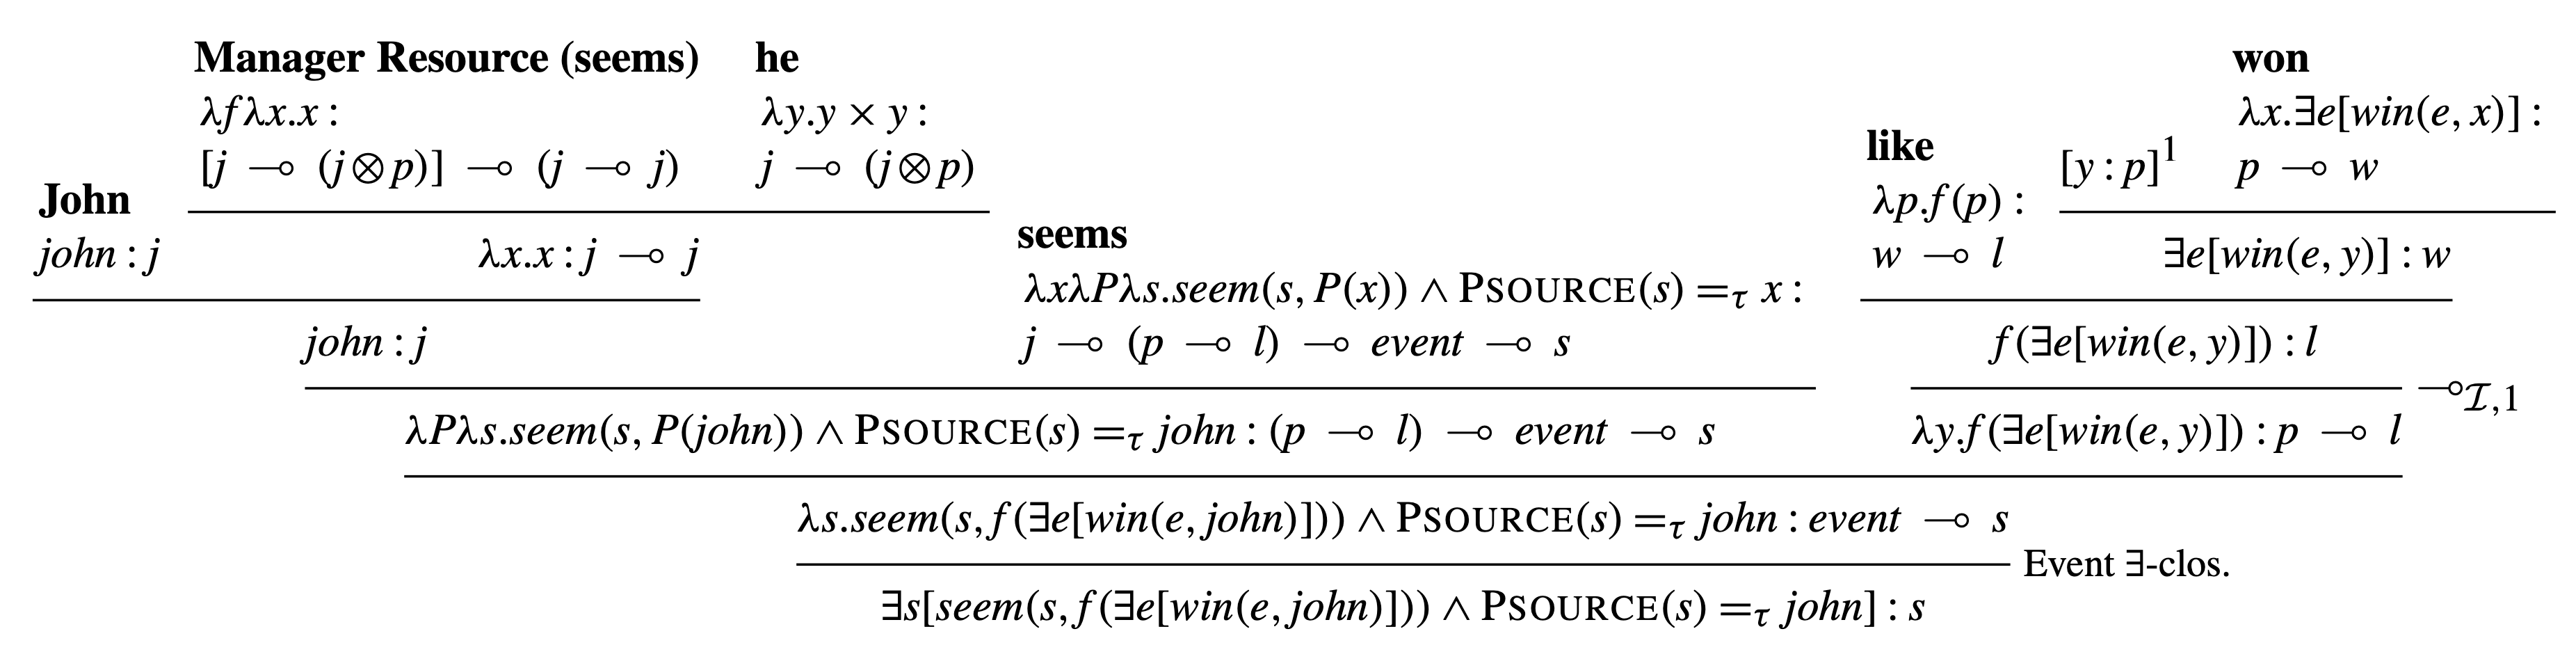
\includegraphics[scale=0.25]{SCR-20240317-bvtm.png}

With something like this, the following more complex Maltese example can also be handled.
\ex. \begingl
  \gla T-i-dhr-u bħallilieku xi ħadd qal-i-l-kom biex t-i-tilq-u //
  \glb 2-\textsc{frm.wl}-appear.\textsc{impv-pl} like.that some no.one say.\textsc{pfv.3sgm-epent.vwl-dat-2pl} in.what 2-\textsc{frm.vwl}-leave.\textsc{impv-pl}//
  \glft `You appear as if someone told you to leave' //
\endgl

Notice the present of both \avm{\1} and \avm{\2}, indicating no syntactic representation of the identity between the matrix subject and the pronoun.
\ex. \avm{[
    pred & `\emph{tidhru} <xcomp>\textsc{subj}' \\
    subj & \1 [
      pred & `\textsc{pro}' \\
      pres & 2 \\
      num & \textsc{pl}
    ] \\
    xcomp & [
      pred & `\emph{bħal} <subj, comp>' \\
      subj & \1 \\
      comp & [
        compform & `\emph{likieku}' \\
        pred & `\emph{qal} <subj, obj\(_{\theta}\), xcomp>' \\
        subj & [
          pred & `\emph{ħadd}' \\
          spec  [
            pred & `\emph{xi}'
          ]
        ] \\
        obj\(_{\theta}\) & \2 [
          pred & `\textsc{pro}' \\
          pers & 2 \\
          num & \textsc{pl} \\
          case & \textsc{dat}
        ] \\
        xcomp & [
          compform & `\emph{biex}' \\
          pred & `\emph{titilqu} <subj>' \\
          subj & \2
        ]
      ]
    ]
]}

\end{document}



